\documentclass[main.tex]{subfiles}

\begin{document}

\section{Why GPUs? What's wrong with CPUs?}
\begin{frame}
  \frametitle{Computing a Matrix Multiplication}
  Let \(A\) and \(B\) be two \(4\times4\) matrices. The matrix multiple \(C = AB\)
  results in another \(4\times4\) matrix.

  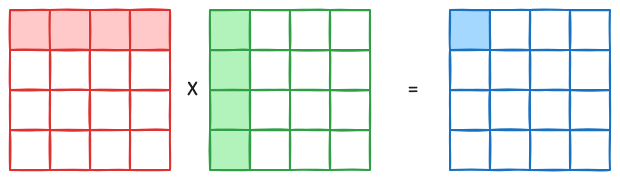
\includegraphics[width=\linewidth]{matmul.png}

  \pause
  \begin{block}{Poor scaling}
    The operations are very simple, but the number of operations grow on the order
    of \(\mathcal{O}(n^3)\), where \(n\) is the dimensions of the matrices.
  \end{block}

  % \begin{block}{Remark}
  %   Linear algebra and matrix multiplications show up everywhere in scientific
  %   computing, so computing them efficiently has always been in high demand.
  % \end{block}
\end{frame}

\begin{frame}[fragile]
  \frametitle{Runtime of a matrix multiplication on a CPU}
  \begin{onlyenv}<1>
    \begin{lstlisting}[
      basicstyle=\ttfamily\small,
      columns=fullflexible,
      breaklines=false,
      breakatwhitespace=false
    ]
for (std::size_t y = 0; y < n; ++y) {
  for (std::size_t x = 0; x < n; ++x) {
    double sum = 0.0;
    for (std::size_t k = 0; k < n; ++k) {
      sum += a[y*n+k] * b[k*n+x];
    }
    c[y*n+x] = sum;
  }
}
    \end{lstlisting}
  \end{onlyenv}

  \begin{onlyenv}<2>
    \centering
    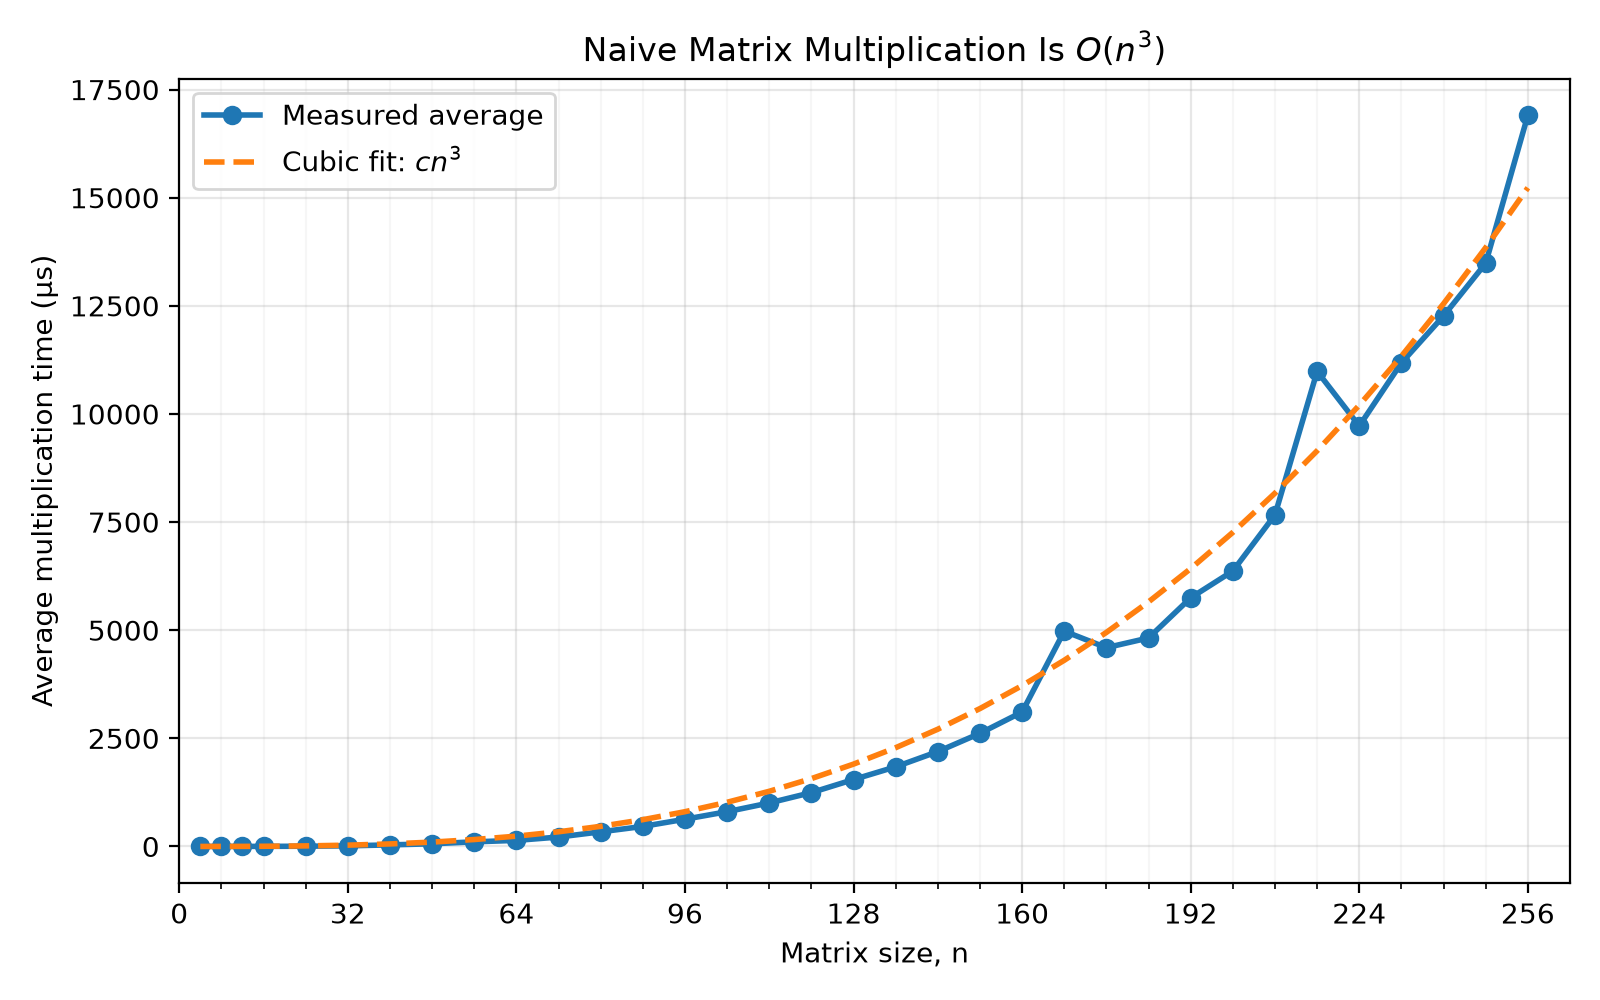
\includegraphics[width=0.9\textwidth]{matmul_timing.png}
  \end{onlyenv}
\end{frame}

\begin{frame}
  \frametitle{Parallelism}
  GPU's came about due to the increase in computational power needed to render
  3D games in real time. This requires \emph{millions} of FLOP's per second.
  CPU's could not keep up.
  Rendering graphics has a nice property that we can take advantage of:
  \textbf{parallelism}.

  Each pixel on the screen doesn't really care any of the other pixels. Furthermore,
  the computation that is required for each pixel isn't that complex either.
  The difficulty in rendering graphics is the volume of computations.

\end{frame}

\begin{frame}
  \frametitle{Matrix Multiplication is Parallel}
  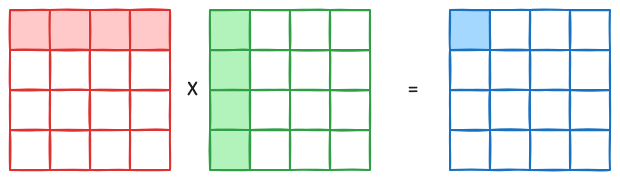
\includegraphics[width=\linewidth]{matmul.png}

  Each element of the output is independent. The results of \(C_{11}\) does not
  effect the results of \(C_{12}\), or any other element.

  \begin{block}{Remark}
    If matrix multiplication is a \textbf{parallel} task, and GPU's were designed for the
    \textbf{parallel} task of rendering graphics, can we repurpose GPU's to do matrix multiplication?
    \pause (Yes.)
  \end{block}
\end{frame}

\begin{frame}
  \frametitle{Takeaway}
  \begin{itemize}
    \item CPUs can't efficiently perform matrix multiplication at scale.
    \item Graphics rendering is a parallel task, and so is matrix multiplication. Thus, GPUs can be good at matrix multiplication.
    \item GEMM is a generalization of of matrix multiplication, and is the operation we will be discussing.
  \end{itemize}

  \begin{block}{Whats next}
    We have established that GPUs \emph{can} do matrix multiplication, but how
    do we actually get there?
  \end{block}
\end{frame}

\end{document}
